\chapter{Diseño del sistema}\label{ch:diseño}
El diseño del sistema define la estructura y organización de los componentes de software necesarios para la operatividad de la aplicación web, estableciendo cómo interactúan y cooperan las tecnologías seleccionadas para cumplir con los requisitos funcionales. Este diseño se ilustra mediante diagramas que muestran la arquitectura y flujo de trabajo del sistema, junto con mockups de interfaz de usuario que proporcionan una visión general de la experiencia e interacción del usuario con la aplicación.

\section{Tabla de tecnologías}
En la tabla \ref{tabla:tabla de tecnologías} se muestra un resumen de las tecnologías usadas dentro de este proyecto. Cada una especifica la tecnología utilizada, su función dentro del proyecto, su categoría y su integración. 
\begin{longtable}{ | c | m{4.5cm} | m{3.5cm} | m{3.5cm} | }
	\rowcolor{black!75}
	\head {Tecnología} & \head {Función} & \head {Categoría} & \head {Integración} \\ \hline
	\endfirsthead
	\multicolumn{4}{c}{{\tablename\ \thetable{} -- continuación}} \\
	\rowcolor{black!75}
	\head {Tecnología} & \head {Función} & \head {Categoría} & \head {Integración} \\ \hline
	\endhead
	\hline \multicolumn{4}{r}{{Continúa en la siguiente página}} \\
	\endfoot
	\hline
	\endlastfoot
	HTML & Lenguaje de marcado para estructura web & Desarrollo Web & Define la estructura de la aplicación \\ \hline
	
	JavaScript & Lenguaje de programación para interactividad & Desarrollo Web & Lógica y funcionalidades interactivas \\ \hline
	
	CSS & Lenguaje para estilización web & Desarrollo Web & Mejora el diseño visual \\ \hline
	
	Angular & Framework para desarrollo web frontend & Desarrollo Web & Gestiona la interfaz y su lógica \\ \hline
	
	Typescript & Superset de JavaScript con tipado estático & Lenguaje de Programación & Facilita el desarrollo seguro en Angular \\ \hline
	
	Tailwind CSS & Framework para estilos CSS utilitario & Estilización Web & Facilita estilos rápidos y responsivos \\ \hline
	
	MathQuill & Renderización de expresiones matemáticas de entrada en páginas web & Matemáticas en aplicaciones web & Captura las fórmulas de entrada del usuario \\ \hline
	
	MathJax & Renderización de fórmulas matemáticas en el sitio web & Matemáticas en aplicaciones web & Mostrar resultados matemáticos correctamente \\ \hline
	
	Node.js & Entorno de ejecución para JavaScript en backend & Desarrollo Web & Procesar cálculos y operaciones backend \\ \hline
	
	Maxima & Software para cálculos algebraicos simbólicos & Matemáticas & Calcular los coeficientes y expansiones de serie \\ \hline
	
	Postman & Herramienta para pruebas de APIs REST & Desarrollo Backend & Valida el funcionamiento del backend \\ \hline
	
	tex2max & Librería para convertir fórmulas TeX a formato Maxima & Parser & Convierte entrada TeX a formato computable \\ \hline
	
	Git & Sistema de control de versiones & Controlador de versiones & Permite gestionar cambios en el código \\ \hline
	
	GitHub & Plataforma para alojar proyectos Git & Controlador de versiones & Almacena y colabora en el repositorio \\ \hline
	
\end{longtable}
\captionof{table}{Tabla de tecnologías y su uso en la aplicación} \label{tabla:tabla de tecnologías}
\vspace{0.5cm}

%HTML, CSS y Javscript son tecnologías base para cualquier apliación web, ya que dan estructura funcionalidad y estilos.  El framework de Angular, en combinación con TypeScript y Tailwind CSS, facilitan un desarrollo web moderno, estructurado y responsivo. MathQuill y MathJax permiten al usuario trabajar con fórmulas matemáticas de manera interactiva tanto al ingresarlas y mostrarlas en el sitio,
%En particular, las tecnologías como HTML, CSS y JavaScript establecen la base para el desarrollo web al definir la estructura, estilización y funcionalidad interactiva de la aplicación. Frameworks como Angular y Tailwind CSS, en combinación con TypeScript, facilitan un desarrollo moderno, estructurado y responsivo. Por otro lado, herramientas como MathQuill y MathJax permiten trabajar con fórmulas matemáticas de manera interactiva, mientras que Maxima y tex2max son fundamentales para cálculos simbólicos y la interpretación de expresiones matemáticas.
%
%Además, Node.js y Postman aseguran la funcionalidad backend y la correcta integración de APIs, mientras que Git y GitHub se emplean para el control de versiones y la colaboración en el código fuente. Esta combinación de tecnologías asegura un flujo de desarrollo eficiente y una aplicación robusta.


\section{Diagrama de arquitectura general del sistema}
El diagrama de  la figura \ref{fig:diagrama_arqui} ilustra la arquitectura general de la apliación de cálculo y graficación mediante el modelo de cliente servidor
\begin{figure}[H]
	\centering
	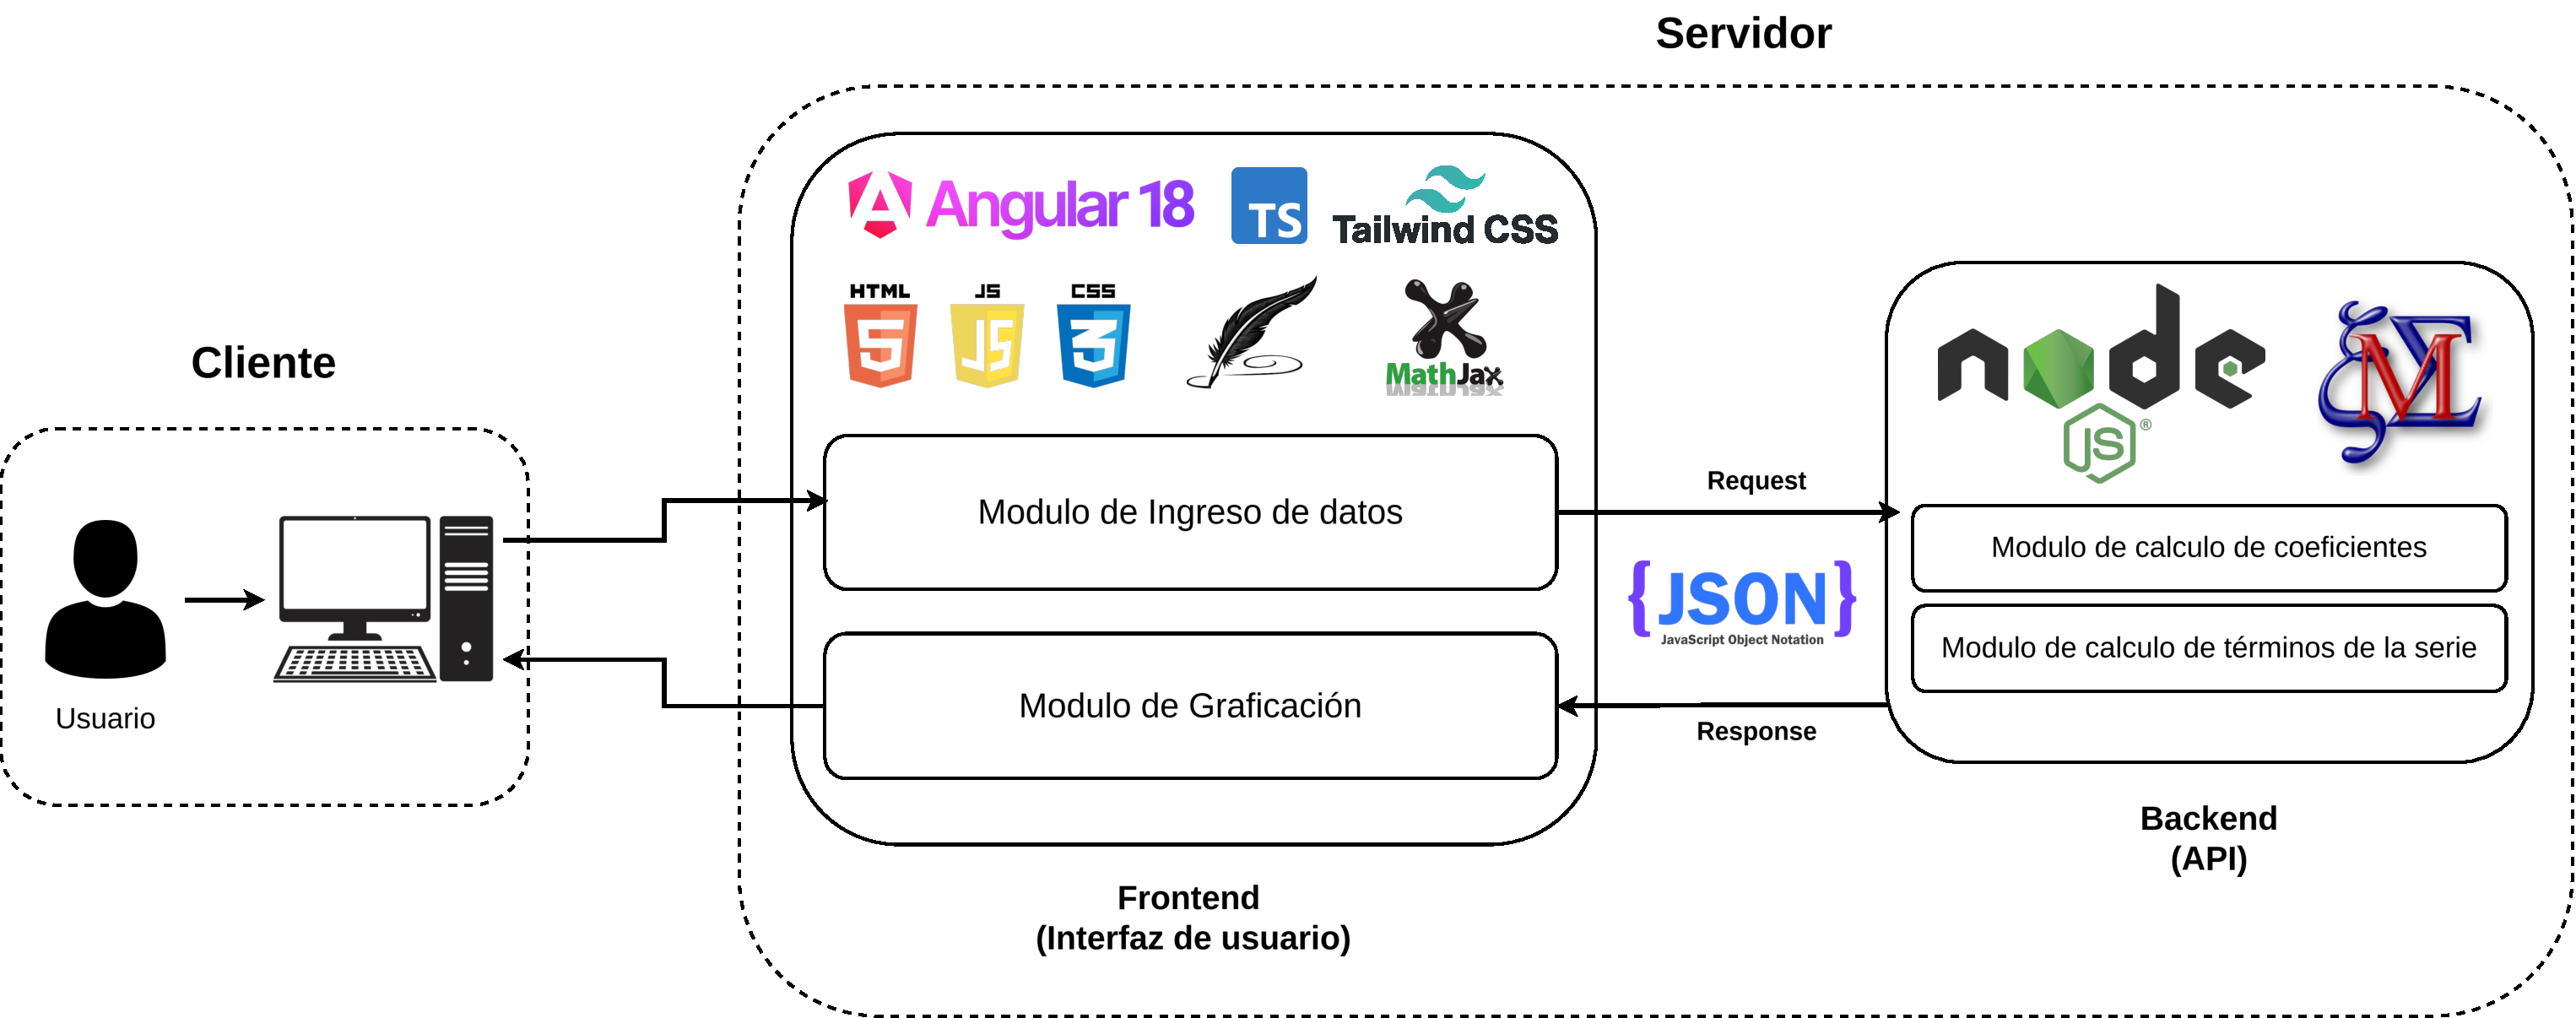
\includegraphics[width=1\textwidth]{img/chapter04/Arquitectura-Sistema-TT.drawio.pdf}
	\caption[Diagrama de arquitectura del sistema.]{Diagrama de arquitectura del sistema. \textit{Fuente: \textit{Elaboración propia}}}
	\label{fig:diagrama_arqui}  % Etiqueta para la figura
\end{figure}
El diagrama de la figura \ref{fig:diagrama_arqui} ilustra la arquitectura general de la aplicación web para el cálculo y graficación de las series de Fourier. Este sistema sigue una arquitectura cliente-servidor, complementada con el modelo de microservicios para garantizar modularidad y escalabilidad en el desarrollo futuro.
\subsection{Arquitectura cliente-servidor}
El sistema se divide en dos componentes principales: el cliente y el servidor.

\begin{itemize}
	\item \textbf{Cliente:}
	\begin{itemize}
		\item El cliente es la interfaz de usuario construida en Angular, donde los usuarios pueden interactuar con el sistema mediante un navegador web.
		\item Incluye los siguientes módulos clave:
		\begin{itemize}
			\item \textbf{Módulo de Ingreso de Datos}: Diseñado para que el usuario ingrese la función \( f \) en términos de $x$ o de $t$, ya sea de manera implícita (función continua) o por partes (trozos de la función). Además, cuenta con herramientas visuales como un botón (\scalebox{0.8}{\faIcon{plus-circle}}) para agregar trozos adicionales o (\scalebox{0.8}{\faIcon{minus-circle}}) para eliminarlos.
			\item \textbf{Módulo de Selección de Parámetros}: Permite configurar el tipo de serie de Fourier que se calculará (trigonométrica, exponencial compleja o extensiones de medio rango). Se presentan las opciones para extensiones pares o impares en caso de la serie trigonométrica.
			\item \textbf{Módulo de Graficación}: Utilizando Canvas, se genera una visualización interactiva de la función original y su aproximación mediante series de Fourier. También incluye controles como un slider para ajustar el número de coeficientes utilizados en la gráfica.
			\item \textbf{MathQuill/MathJax}: Herramientas integradas para que el usuario pueda capturar las funciones y la apliación muestre los resultados en un formato amigable utilizando notación TeX.
			\item \textbf{tex2max}: Se parsean todas las entradas necesarias (la función y sus intervalos) para ser enviadas al servidor y realizar los cálculos. 
		\end{itemize}
	\end{itemize}
	
	\item \textbf{Servidor:}
	\begin{itemize}
		\item El servidor está implementado en NodeJS y se comunica con el cliente a través de una API RESTful.
		\item Se encarga de procesar las solicitudes enviadas desde el cliente y realizar  el calculo de los coeficientes y la extensión de la serie mediante el sistema algebraico computacional (CAS) Maxima. Además de también convertir estas expresiones a formato de Tex.
		\item Principales responsabilidades:
		\begin{itemize}
			\item Recepción y parseo de las entradas en formato JSON, enviadas desde el cliente con la ayuda de la librería tex2max.
			\item Ejecución de comandos en Maxima para calcular las integrales definidas y obtener los coeficientes \( a_0 \), \( a_n \), \( b_n \) (para la serie trigonométrica) o \( c_n \) (para la exponencial compleja). Además de almacenar estos resultados en formato Maxima y en formato Tex
			\item Generación de resultados en formato JSON para su devolución al cliente, incluyendo los coeficientes calculados y las series de Fourier en formato Maxima y Tex.
			
		\end{itemize}
	\end{itemize}
\end{itemize}
\subsection{Arquitectura basada en microservicios}
Aunque actualmente solo se cuenta con un microservicio (el API para cálculo de series de Fourier), el diseño sigue una arquitectura de microservicios para permitir la escalabilidad futura. Esto implica que:

\begin{itemize}
	\item El servicio de cálculo de series de Fourier está desacoplado del resto del sistema, permitiendo su mantenimiento, actualización o reemplazo sin afectar otras partes de la aplicación.
	\item En el futuro, se pueden agregar otros microservicios para cálculos relacionados sin alterar la arquitectura actual.
	\item Cada microservicio puede ser independiente y comunicarse con el servidor principal mediante una API RESTful bien definida.
\end{itemize}

\subsection{Descripción del Diagrama}

En el diagrama de la figura \ref{fig:diagrama_arqui}:

\begin{itemize}
	\item \textbf{Cliente}: Representa al usuario final que interactúa con el sistema a través de un navegador web. Incluye herramientas de ingreso de datos, selección de parámetros y graficación interactiva.
	\item \textbf{Servidor}: Implementado en NodeJS, actúa como intermediario entre el cliente y el sistema de cálculo matemático Maxima. Maneja las solicitudes entrantes, procesa los cálculos y devuelve los resultados.
	\item \textbf{Maxima}: Es el motor de cálculo algebraico que realiza las operaciones matemáticas necesarias para obtener los coeficientes y las series de Fourier.
	\item \textbf{JSON}: Actúa como formato estándar para la comunicación entre el cliente, el servidor y los microservicios, asegurando interoperabilidad y facilidad de integración.
\end{itemize}

\newpage

\section{Diagramas de secuencia UML}
Los diagramas de secuencia UML son una representación gráfica que ilustra la interacción de objetos en un sistema de forma cronológica, capturando la secuencia de mensajes intercambiados entre objetos y el orden en que ocurren estas interacciones.


%inkscape img/chapter04/DS2.svg --export-filename=img/chapter04/DS2.pdf
\subsection{Ingreso y validación de una función}
El diagrama de  la figura \ref{fig:Diagrama_secuencia_1} ilustra como el usuario ingresa una función, donde esta función puede estar formada de múltiples trozos y el usuario puede añadir o quitar estos trozos, definiendo su valor además del intervalo en el que está definido. Estos datos validarán para indicar si se ingresó algún valor o función no válidos. También ingresará el tipo de extensión de la serie.
\begin{figure}[H]
	\centering
	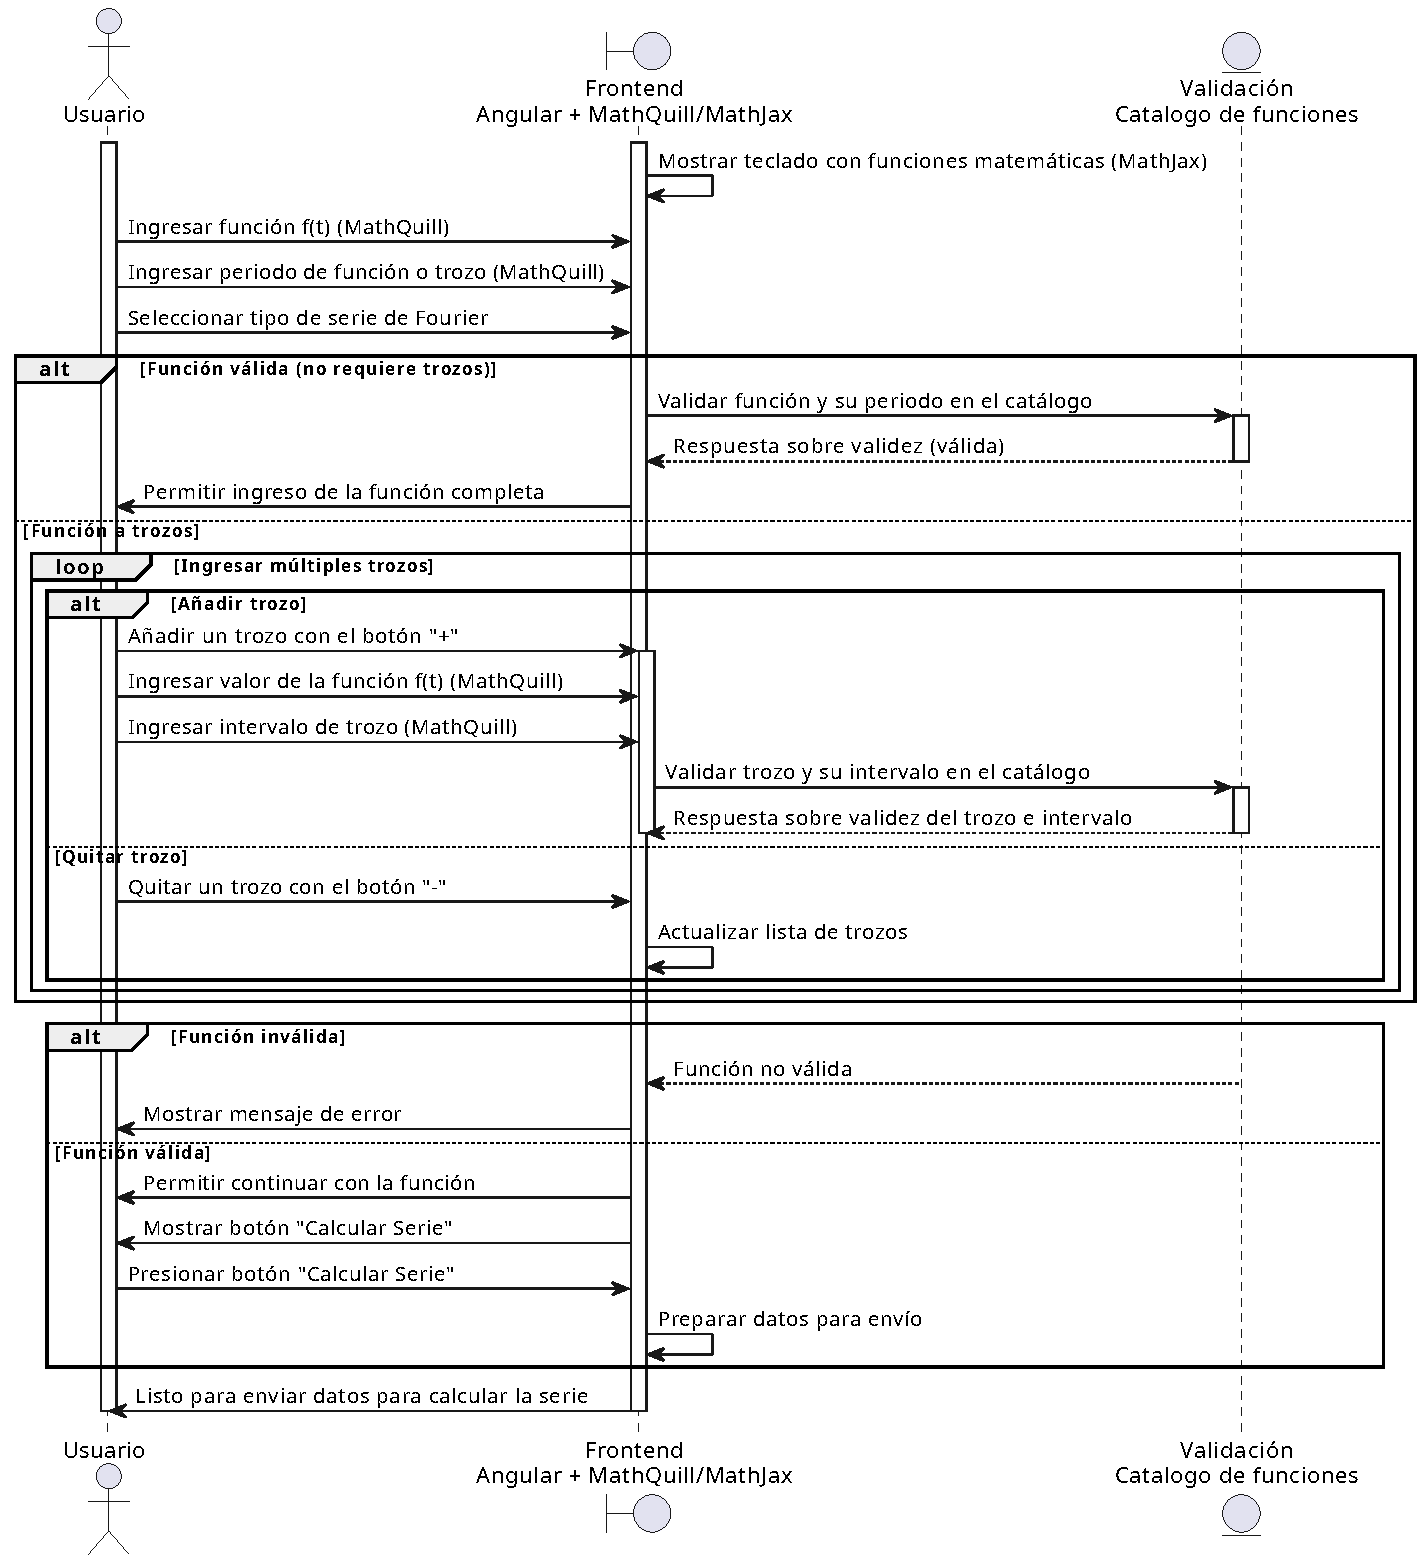
\includegraphics[width=1\textwidth]{img/chapter04/DS1.pdf}
	\caption[Diagrama de Secuencia 1.]{Diagrama de Secuencia 1. \textit{Fuente: \textit{Elaboración propia}}}
	\label{fig:Diagrama_secuencia_1}
\end{figure}


\subsection{Parseo de función para la API}
El diagrama de  la figura \ref{fig:Diagrama_secuencia_2} ilustra como, una vez confirmada la función ingresada por el usuario, se parsea la expresión y sus intervalos de formato LaTeX y a Maxima utilizando la librería de parseo. Luego, los datos se estructuran en JSON indicando la función, sus intervalos y el tipo de extensión y se envían al la API para realizar los cálculos.
\begin{figure}[H]
	\centering
	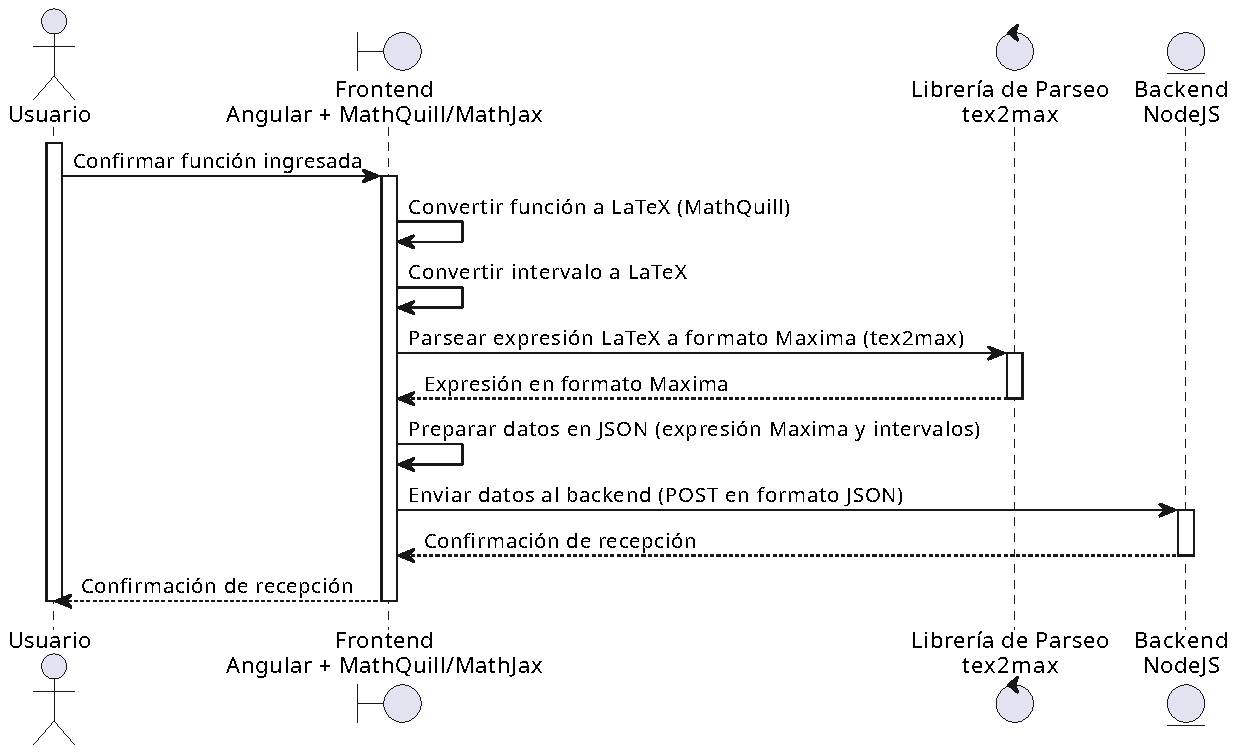
\includegraphics[width=1\textwidth]{img/chapter04/DS2.pdf}
	\caption[Diagrama de Secuencia 2.]{Diagrama de Secuencia 2. \textit{Fuente: \textit{Elaboración propia}}}
	\label{fig:Diagrama_secuencia_2}
\end{figure}

 \newpage
 
\subsection{Cálculo de la Serie de Fourier en la API}
En el diagrama de  la figura \ref{fig:Diagrama_secuencia_3} se detalla el proceso en la API para calcular la serie de Fourier. Dependiendo del tipo de serie seleccionado (trigonométrica o exponencial), se calculan los coeficientes correspondientes. Se realizan integraciones en cada intervalo si la función es a trozos y finalmente se generan los resultados, tanto en formato Maxima como en formato LaTeX para su visualización.
\begin{figure}[H]
	\centering
	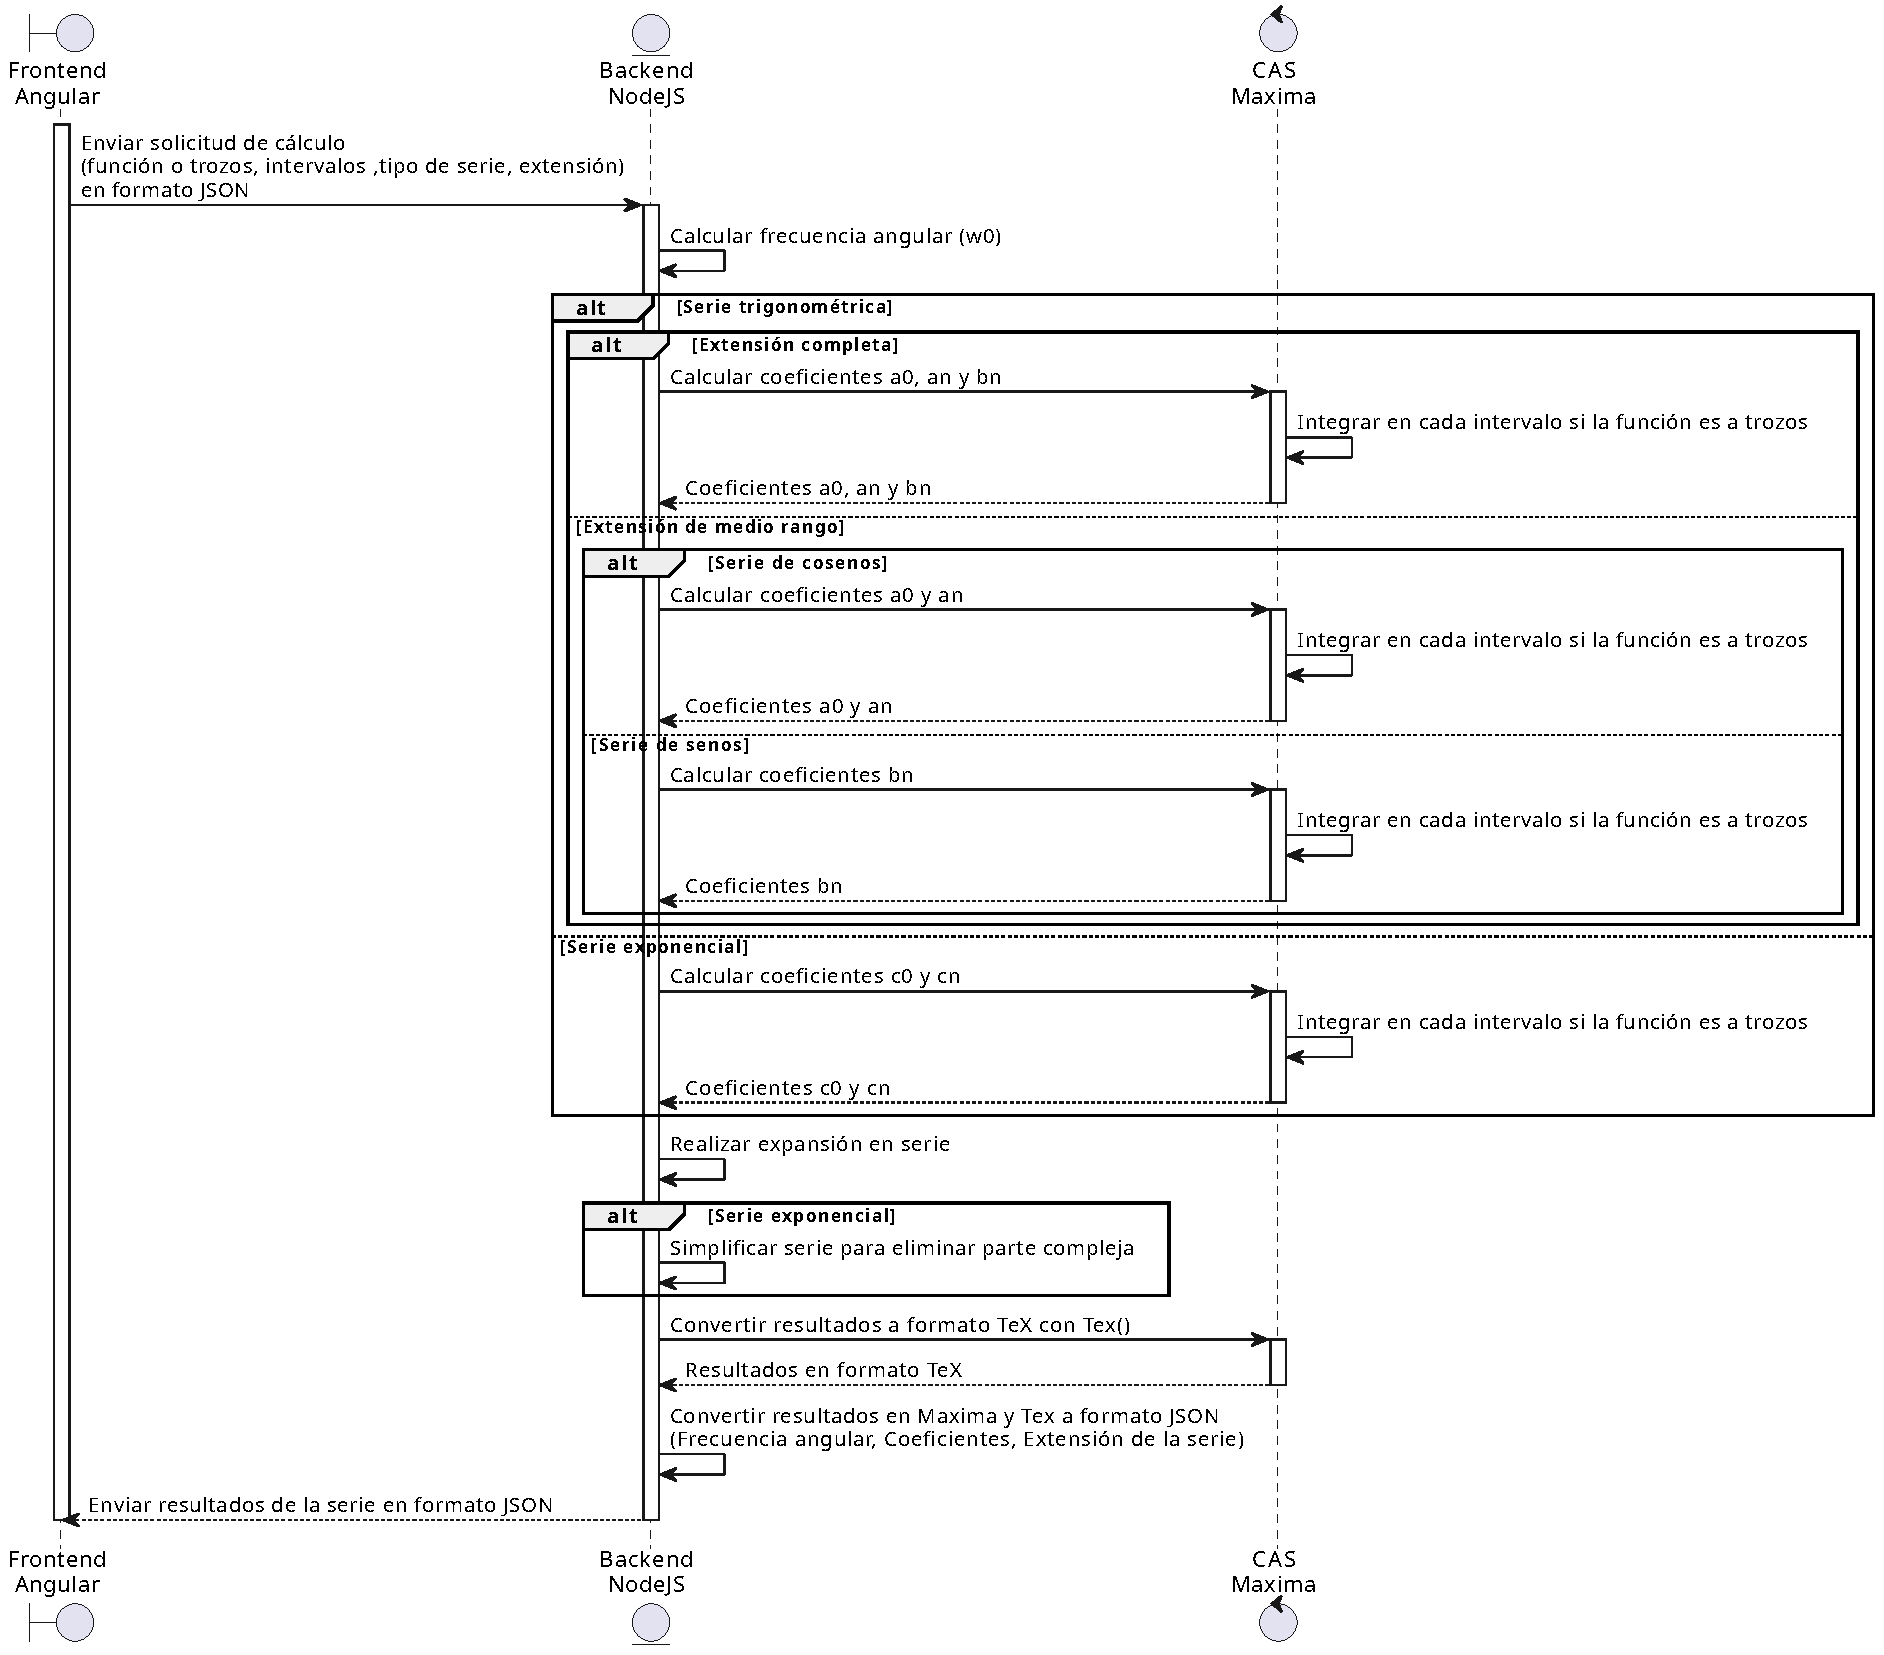
\includegraphics[width=1\textwidth]{img/chapter04/DS3.pdf}
	\caption[Diagrama de Secuencia 3.]{Diagrama de Secuencia 3. \textit{Fuente: \textit{Elaboración propia}}}
	\label{fig:Diagrama_secuencia_3}
\end{figure}

\newpage

\subsection{Preparación de resultados para visualización}
El diagrama de  la figura \ref{fig:Diagrama_secuencia_4} muestra cómo se preparan los resultados para su visualización en el frontend. Los datos recibidos del backend en formato JSON se deserializan y se convierten en formatos JavaScript y LaTeX, listos para ser consumidos por el usuario en diferentes para la graficación y ver los resultados en su notación matemática, respectivamente.
\begin{figure}[H]
	\centering
	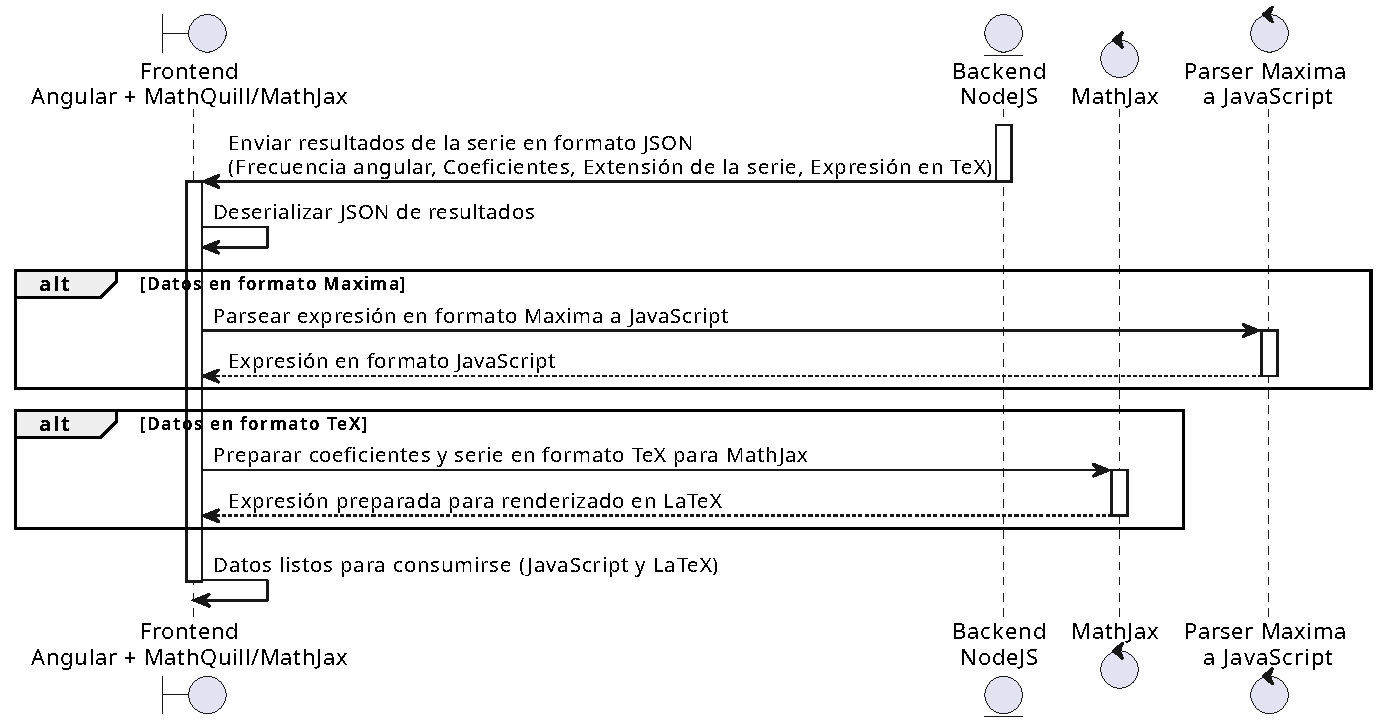
\includegraphics[width=1\textwidth]{img/chapter04/DS4.pdf}
	\caption[Diagrama de Secuencia 4.]{Diagrama de Secuencia 4. \textit{Fuente: \textit{Elaboración propia}}}
	\label{fig:Diagrama_secuencia_4}
\end{figure}

\newpage

\subsection{Visualización de los resultados e interactividad con la gráfica}
El diagrama de  la figura \ref{fig:Diagrama_secuencia_5} representa cómo el frontend toma los resultados para para graficar la serie de Fourier de manera interactiva, permitiendo al usuario ajustar el número de términos y ver la actualización de la gráfica en tiempo real. Además, los coeficientes y el resultado en forma de serie se muestran en formato matemático usando MathJax.
\begin{figure}[H]
	\centering
	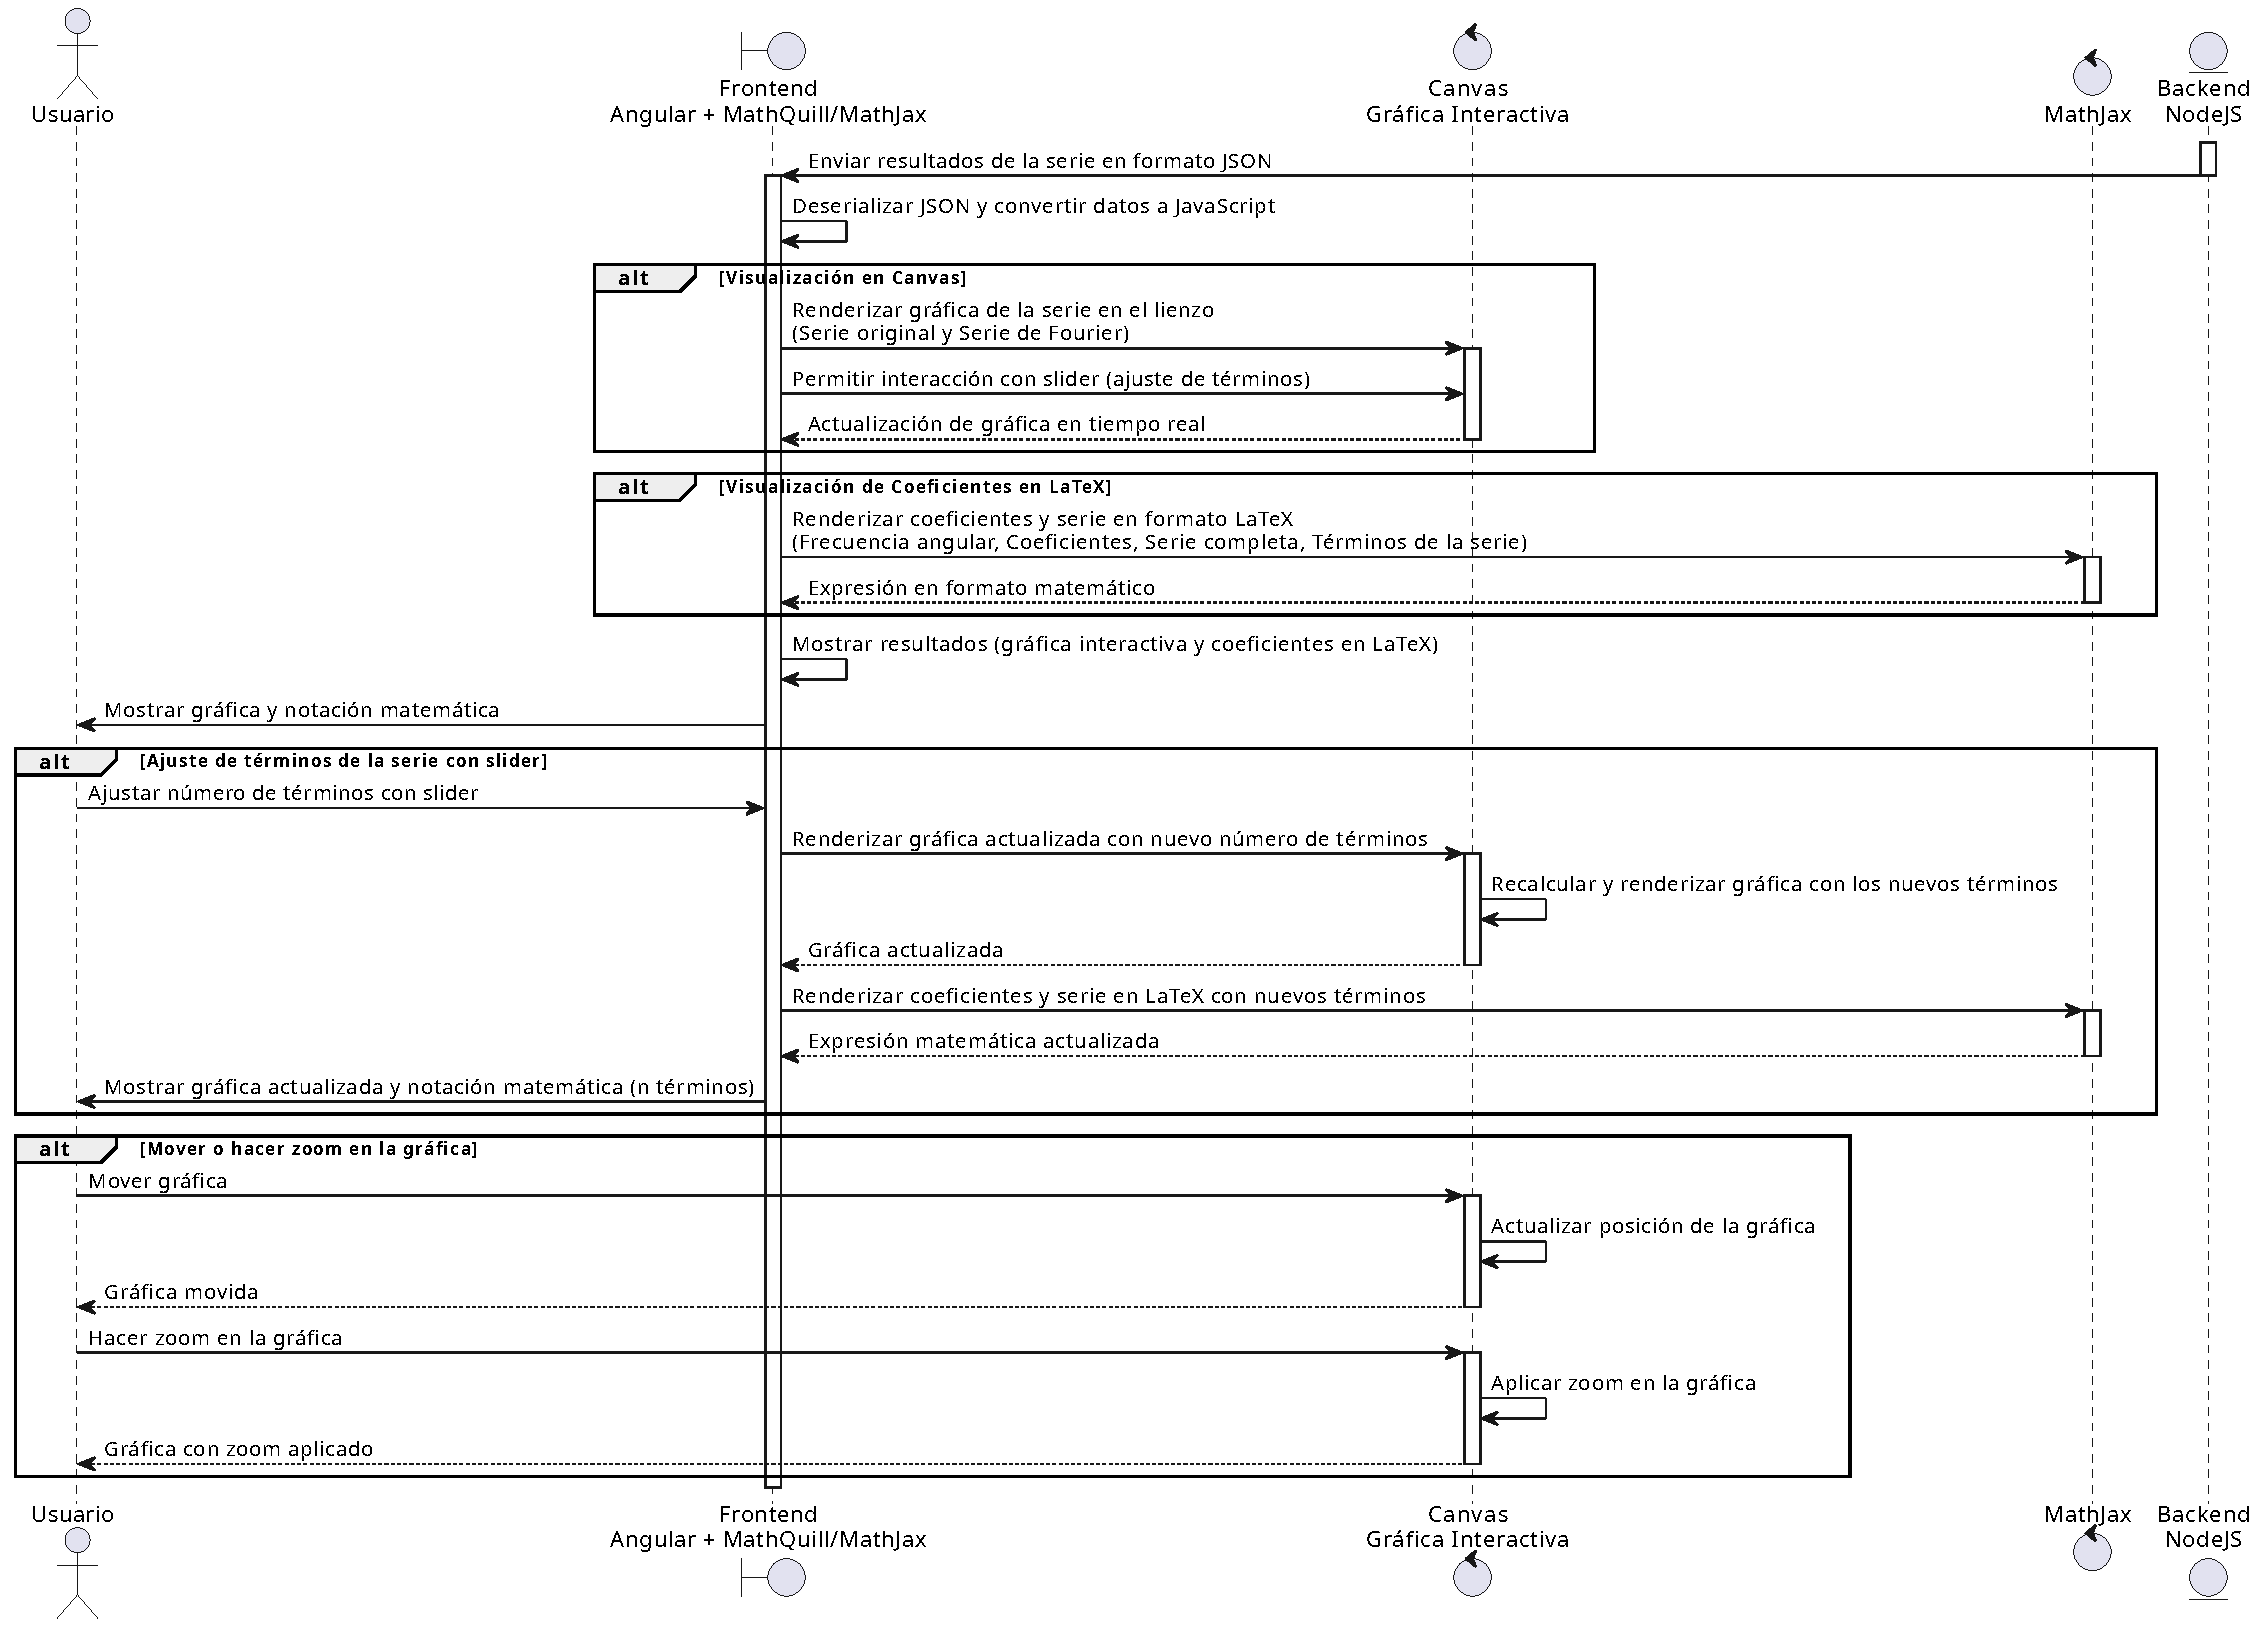
\includegraphics[width=1\textwidth]{img/chapter04/D5-6.pdf}
	\caption[Diagrama de Secuencia 5.]{Diagrama de Secuencia 5. \textit{Fuente: \textit{Elaboración propia}}}
	\label{fig:Diagrama_secuencia_5}
\end{figure}

\newpage

\section{Diagramas de clases UML}
A pesar de que este proyecto no utiliza el paradigma de programación orientada a objetos (POO), se maneja un objeto que es crucial para la comunicación entre el cliente y el servidor, el JSON, ya que se usa como un objeto de transferencia de datos. Para la arquitectura planteada para el proyecto, se cuenta con dos JSON, el que envía el cliente al servidor (Request) y el que envía el servidor al cliente (Response). 

\subsection{Diagrama de clases ClientRequest}
ClientRequest es la clase principal que representa el JSON que el cliente envía al servidor, en el, se captura toda la información necesaria para que el servidor pueda calcular la serie de Fourier solicitada. \newline

La estructura de la clase principal \texttt{ClientRequest} y sus relaciones es la siguiente:

\begin{figure}[H]
	\centering
	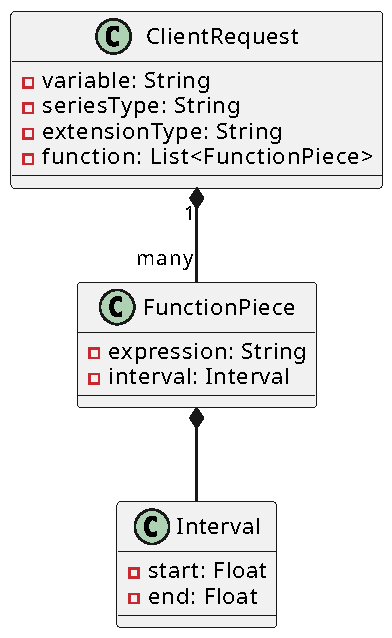
\includegraphics[width=0.5\textwidth]{img/chapter04/DC_JSON_Client.pdf}
	\caption[Diagrama de clases del JSON del cliente.]{Diagrama de clases del JSON del cliente. \textit{Fuente: \textit{Elaboración propia}}}
	\label{fig:Diagrama_clase_cliente}
\end{figure}


En donde la clase principal \textbf{ClientRequest} tiene los siguientes atributos:
\begin{itemize}
	\item \texttt{variable}: La variable independiente de la función (\texttt{String}).
	\item \texttt{seriesType}: El tipo de Serie de Fourier (\texttt{String}). Por ejemplo, \texttt{trigonometric} o \texttt{complex}.
	\item \texttt{extensionType}: Define si es una extensión par, impar o periódica (\texttt{String}). Por ejemplo, \texttt{odd} o \texttt{even}.
	\item \texttt{function}: Lista de objetos \texttt{FunctionPiece} que representan los trozos de la función (\texttt{List<FunctionPiece>}).
\end{itemize}

	
La clase \textbf{FunctionPiece} tiene los siguientes atributos: 
\begin{itemize}
	\item \texttt{expression}: La expresión matemática de un segmento de la función (\texttt{String}).
	\item \texttt{interval}: Objeto de tipo \texttt{Interval} que define el intervalo de validez del segmento.
\end{itemize}

	
La clase  \textbf{Interval} tiene los siguientes atributos:
\begin{itemize}
	\item \texttt{start}: Inicio del intervalo (\texttt{Float}).
	\item \texttt{end}: Fin del intervalo (\texttt{Float}).
\end{itemize}

Las relaciones que se tienen en estas clases son:
\begin{itemize}
	\item \texttt{ClientRequest} tiene una relación de composición con \texttt{FunctionPiece}, indicando que un \texttt{ClientRequest} puede contener múltiples segmentos de función.
	\item \texttt{FunctionPiece} tiene una relación de composición con \texttt{Interval}, indicando que cada segmento de función tiene un intervalo definido.
\end{itemize}



\subsection{Diagrama de clases ServerResponse}
ServerResponse es la clase principal que representa el JSON que el servidor devuelve al cliente después de calcular la Serie de Fourier. \newline
La estructura de la clase principal \texttt{ServerResponse} es la siguiente:
\begin{figure}[H]
	\centering
	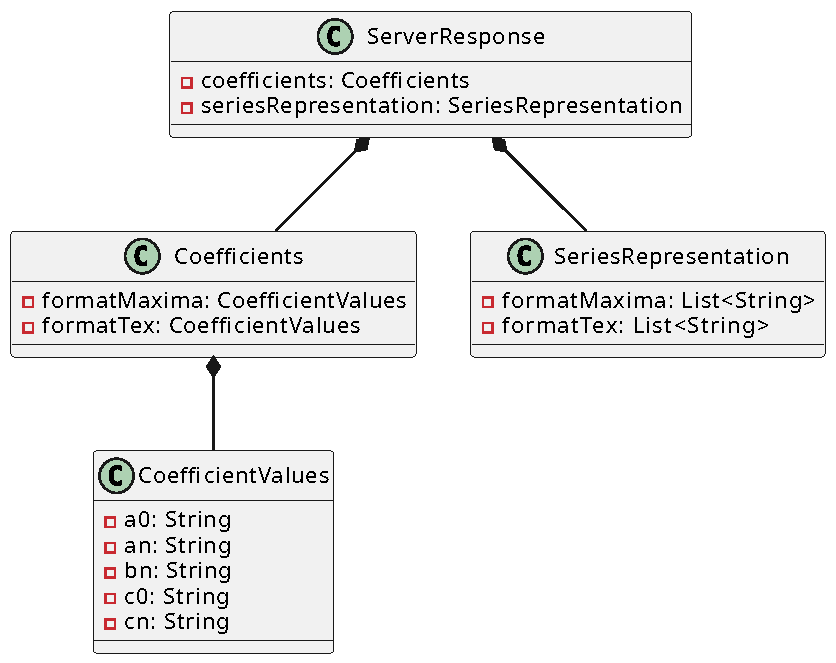
\includegraphics[width=0.75\textwidth]{img/chapter04/DC_JSON_Server.pdf}
	\caption[Diagrama de clases del JSON del servidor.]{Diagrama de clases del JSON del servidor. \textit{Fuente: \textit{Elaboración propia}}}
	\label{fig:Diagrama_clase_servidor}
\end{figure}

En donde la clase principal \textbf{ServerResponse} tiene los siguientes atributos:
\begin{itemize}
	\item \texttt{coefficients}: Objeto de tipo \texttt{Coefficients} que contiene los valores de los coeficientes calculados.
	\item \texttt{seriesRepresentation}: Objeto de tipo \texttt{SeriesRepresentation} que incluye las representaciones de la serie calculada.
\end{itemize}


La clase \textbf{Coefficients} tiene los siguientes atributos: 
\begin{itemize}
	\item \texttt{formatMaxima}: Objeto de tipo \texttt{CoefficientValues} que contiene los coeficientes en formato Maxima.
	\item \texttt{formatTex}: Objeto de tipo \texttt{CoefficientValues} que contiene los coeficientes en formato LaTeX.
\end{itemize}


La clase \textbf{CoefficientValues} tiene los siguientes atributos:
\begin{itemize}
	\item \texttt{a0}: Coeficiente promedio constante  (\texttt{String}).
	\item \texttt{an}: Coeficiente para los componentes coseno (\texttt{String}).
	\item \texttt{bn}: Coeficiente para los componentes seno (\texttt{String}).
	\item \texttt{c0}: Coeficiente promedio constante complejo (\texttt{String}).
	\item \texttt{cn}: Coeficiente complejo (\texttt{String}).
\end{itemize}


La clase \textbf{SeriesRepresentation} tiene los siguientes atributos:
\begin{itemize}
	\item \texttt{formatMaxima}: Representación de la serie en formato Maxima (\texttt{List<String>}).
	\item \texttt{formatTex}: Representación de la serie en formato LaTeX (\texttt{List<String>}).
\end{itemize}


Las relaciones que se tienen en estas clases son:
\begin{itemize}
	\item \texttt{ServerResponse} tiene una relación de composición con \texttt{Coefficients} y \texttt{SeriesRepresentation}.
	\item \texttt{Coefficients} tiene una relación de composición con \texttt{CoefficientValues}, indicando que contiene coeficientes en diferentes formatos.
\end{itemize}
Estos dos diagramas nos dan la estructura de como es que los datos que se envían y reciben entre el cliente y el servidor.

\newpage

\section{Diagrama de casos de uso}
En la figura \ref{fig:Diagrama_casos_de_uso} se presenta el diagrama de casos de uso general de la aplicación, el cual describe las interacciones entre el usuario y las principales funcionalidades del sistema. 
\begin{figure}[H]
	\centering
	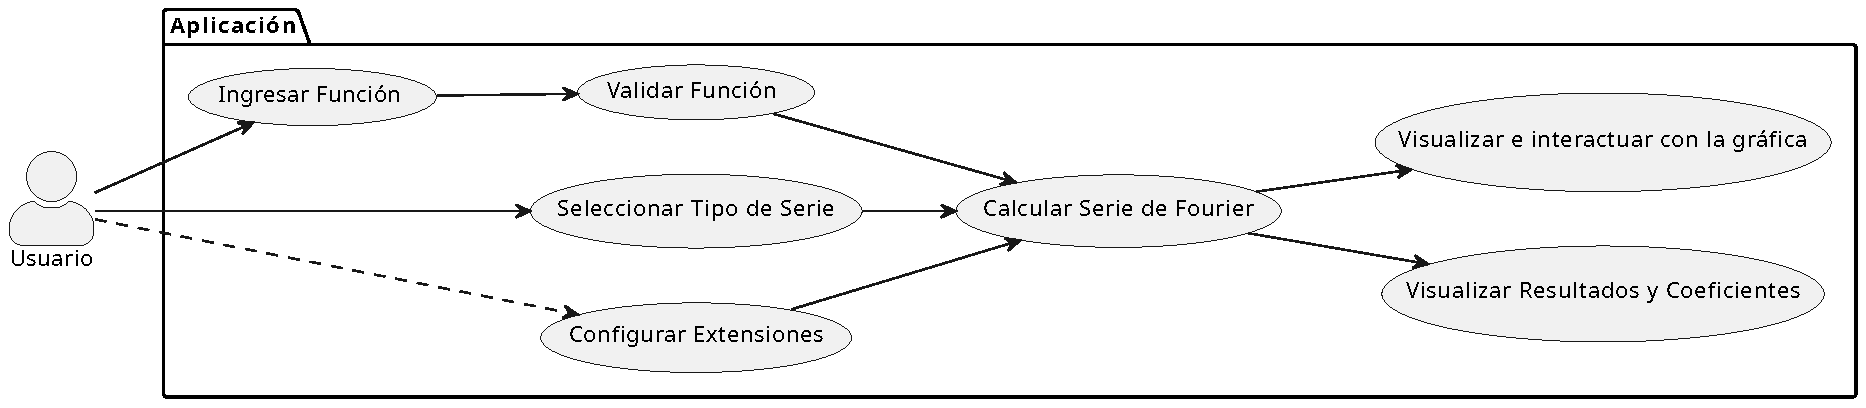
\includegraphics[width=1\textwidth]{img/chapter04/DCU.pdf}
	\caption[Diagrama general de casos de uso del sistema]{Diagrama general de casos de uso del sistema. \textit{Fuente: \textit{Elaboración propia}}}
	\label{fig:Diagrama_casos_de_uso}
\end{figure}
El flujo del diagrama inicia con el ingreso de la función y la validación de esta. Opcionalmente, el usuario puede configurar extensiones de medio rango si la serie seleccionada es trigonométrica. Posteriormente, se calcula la Serie de Fourier, y el usuario puede visualizar los resultados numéricos de los coeficientes o interactuar con la gráfica generada.


\section{Diseño de la Interfaz de Usuario}
\subsection{Estructura de la Interfaz}
